\documentclass{article}
\usepackage[utf8]{inputenc}
\usepackage{commath}
\usepackage{graphicx}

\title{Iskanje po zbirski dokumentov -
        Latentno semantično indeksiranje \\
        \large Matematično modeliranje, projektna naloga}
\author{Nedžad Beus, Gašper Spagnolo, Tilen Ožbot}
\date{Junij 2022}

\begin{document}

\maketitle
\pagebreak

% PRVA STRAN
\section{Opis naloge}
\par Naloga je izdelati program, ki bo v zbirki dokumentov za dane ključne besede poiskal najbolj relevantne dokumente, s pomočjo metode \textit{latentnega semantičnega indeksiranja} (LSI). 
\par LSI je metoda za indeksiranje in iskanje, ki uporablja dekompozicijo singularnih vrednosti (SVD) za prepoznavanje vzorcev v odnosih med izrazi in pojmi v nestrukturirani zbirki besedil. Metoda temelji na načelu, da imajo besede, ki se uporabljajo v istem kontekstu, podoben pomen. Ključna značilnost LSI je, da lahko izlušči konceptualno vsebino besedila z vzpostavljanjem povezav med izrazi, ki se pojavljajo v podobnih kontekstih.

\section{Resitev}
Nalogo razdelimo na več korakov:

\subsection{Izdelava začetne matrike}
Iz zbirke dokumentov zgradimo matriko A povezav med besedami in dokumenti. Vsakemu dokumentu v zbirki ustreza stolpec v matriki, vsaki besedi v zbirki pa vrstica. Element $a_{ij}$ naj v začetku predstavlja frekvenco \textit{i}-te besede v \textit{j}-tem dokumentu.

\textbf{Enostaven primer:}\\
Imejmo tri dokumente:

\begin{itemize}
    \item $d1:$ Jogurt je v vrecki.
    \item $d2:$ V vrecki imam jogurt.
    \item $d3:$ Zunaj piha veter.
\end{itemize}

Najprej prestejemo pojavitve besed v vseh dokumentih.

\[
\begin{tabular}{ |c|c|c|c| } 
    \hline
    beseda    & d1 &  d2  & d3\\
    \hline
    "jogurt"    & 1 & 1 & 0 \\ 
    "je"        & 1 & 0 & 0 \\ 
    "v"         & 1 & 1 & 0 \\ 
    "vrecki"    & 1 & 1 & 0 \\ 
    "imam"      & 1 & 0 & 0 \\ 
    "zunaj"     & 0 & 0 & 1 \\ 
    "piha"      & 0 & 0 & 1 \\ 
    "veter"     & 0 & 0 & 1 \\ 
    \hline
\end{tabular}
\]

Nato lahko zgradimo matriko $A$:

\[
A = \begin{bmatrix}
        1 & 1 & 0 \\
        1 & 0 & 0 \\
        1 & 1 & 0 \\
        1 & 1 & 0 \\
        1 & 0 & 0 \\
        0 & 0 & 1 \\
        0 & 0 & 1 \\       
        0 & 0 & 1 \\
 \end{bmatrix}
\]

\par Metodo in s tem rezultate lahko izboljšamo, če elemente matrike $a_{ij}$ izračunamo z bolj kompleksnimi merami kot so npr. entropija. Element matrike $a_{ij}$ lahko zapisemo kot
\[ a_{ij} = l_{ij} \cdot g_i,\]
kjer je $L_{ij}$ lokalna mera za pomembnost besede v dokumentu, $G_i$ pa globalna mera pomembnosti besede.
\[ L_{ij} = log(f_{ij} + 1)\]
\[ G_i = 1 - \sum_{j} \frac{p_{ij} log(p_{ij})}{logn} \]
\[ p_{ij} = \frac{f_{ij}}{gf_i},\]
kjer je $f_{ij}$ frekvenca \textit{i}-te besede v \textit{j}-tem dokumentu, $gf_i$ pa globalna frekvenca \textit{i}-te besede v bazi dokumentov. 
\par \textbf{Primer matrike $A$ z uporabo entropije:}
\[
A = \begin{bmatrix}
    1.6309  & 1.6309 &  0 \\
    1.0000  & 0      &  0 \\
    1.6309  & 1.6309 &  0 \\
    1.6309  & 1.6309 &  0 \\
    0       & 1.0000 &  0 \\
    0       & 0      &  1.0000 \\
    0       & 0      &  1.0000 \\
    0       & 0      &  1.0000 \\
 \end{bmatrix}
\]

\subsection{Razcep matrike}
\par Matriko A razcepimo z odrezanim SVD razcepom A = $U_kS_kV_k^T$, ki obdrži le \textit{k} največjih singularnih vrednosti. Stolpci matrike $U_k$ nam predstavljo t.i. vektorje izrazov, stolpci matrike $V_k$ pa t.i. vektorje dokumentov. S odstranjitvijo najmanjših singularnih vrednosti skušamo aproksimirati originalno matriko A in s tem zmanjšati šum. Število \textit{k} je odvisno od velikosti baze podatkov (npr. pri 1000+ dokumentih je \textit{k}=100 dobra aproksimacija).
\par \textbf{Primer razcepa matrike $A$ z uporabo entropije:}

\[
A = \begin{bmatrix}
    0.5601 &       0 & -0.0000 \\ 
   0.1717 &   0.0000 &  0.7071 \\
   0.5601 &        0 & -0.0000 \\
   0.5601 &        0 & -0.0000 \\
   0.1717 &  -0.0000 & -0.7071 \\
  -0.0000 &   0.5774 &  0.0000 \\
  -0.0000 &   0.5774 &  0.0000 \\
  -0.0000 &   0.5774 &  0.0000 \\
 \end{bmatrix}
 \begin{bmatrix}
    4.1182 &        0 &        0 \\ 
        0  &   1.7321 &        0 \\
        0  &        0 &   1.0000 \\
 \end{bmatrix}
 \begin{bmatrix}
     7.0711e^{-01} &   7.8505e^{-17} &  7.0711e^{01} \\ 
     7.0711e^{-01} &   1.9626e^{-16} & -7.0711e^{01} \\
   -2.3551e^{-16} &   1.0000         & -7.8505e^{-17} \\
 \end{bmatrix}
\]

\subsection{Vektor poizvedbe}
\par Besede po katerih želimo iskati oz. iskalni niz lahko zapišemo z vektorjem \textit{q}, ki je enake dolžine kot število vrstic v matriki A. Iskalni niz tretiramo kot dokument. Iz iskalnega niza generiramo vektor v prostoru dokumentov po naslednji formuli:
\[ \hat{q} = q^TU_kS_k^{-1},\]
ki jo izpeljemo iz naslednjih formul:
\[ A = USV^T,\]
\[ A^T = (USV^T)^T = VSU^T\]
\[ A^TUS^{-1} = VSU^TUS^{-1},\]
\[ V = A^TUS^{-1},\]
\[ \hat{q} = q^TUS^{-1}.\]
\par Dobljeni vektor $\hat{q}$ je v enakem prostoru kot stolpci v matriki $V_k$. Dokumenti oz. stolpci matrike $V_k$, ki najbolj ustrezajo poizvedbi so tisti, ki so dovolj blizu vektorju $\hat{q}$. Za razdaljo uporabimo kosinus kota med vektorjem. 
\[ cos(\alpha) = \frac{\hat{q} \cdot \Vec{v_i}}{\norm{\hat{q}} \cdot \norm{\Vec{v_i}}}\]

\section{Rezultati}
Za bazo podatkov smo se odločili za recepte jedi.
% nasi podatki, predstavimo rezultate, razlicni k-ji itd.

\section{Dodajanje dokumentov in besed}
Predpostavimo, da je začetna matrika že zgrajena in SVD te matrike izračunan. Če želimo dodati nove dokumente oz. nove besede, obstajata dve možnosti za dodajanje:
\begin{enumerate}
    \item ponovno generiranje začetne matrike in izračunavanje SVD,
    \item metoda \textit{folding-in} ali zgibanje, ki je hitrejša.
\end{enumerate}
\subsection{Ponovno izračunavanje SVD}
 Za to možnost se odločimo, ko dodamo veliko število dokumentov oz. besed. Ponovno zgradimo začetno matriko in SVD razcep. Ponovni izračun SVD-ja omogoča, da nove besede in dokumenti neposredno vplivajo na latentno semantično strukturo, saj se ustvari nova začetna matrika in s tem drugačen SVD razcep. Slabost je, da ponovno izračunavanje SVD velike matrike zahteva veliko časa in pomnilnika.
\subsection{Metoda \textbf{folding-in} ali zgibanje}
\par Metoda zgibanja temelji na obstoječi latentni semantični strukturi, trenutni matriki, zato nove besede in dokumenti ne vplivajo na prestavitev ze obstoječih izrazov in dokumentov. Ta metoda zahteva manj časa in pomnilnika, vendar lahko poslabša prestavitev novih izrazov in dokumentov.
\par Postopek je enak postopku za vektor poizvedbe. Vsak nov dokument je predstavljen kot utežena vsota njegovih sestavnih vektorjev izrazov.
\[ \hat{d} = d^TU_kS^{-1}_k\]
Izračunan vektor je dodan naboru obstoječih vektorjev dokumentov ali stolpcev v matriki $V_k$. \\

% slika
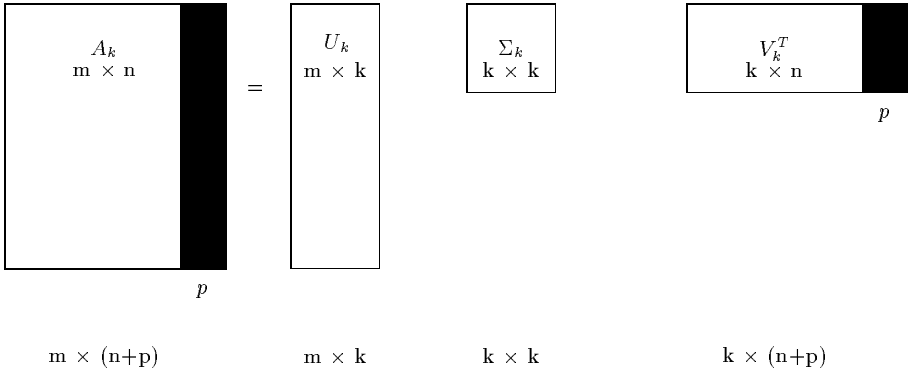
\includegraphics[scale=0.5]{assets/zaDokumente.png}
\\
\par Podobno lahko nove besede izrazimo kot uteženo vsoto vektorjev dokumentov, v katerih se pojavljajo.
\[ \hat{t} = tV_kS^{-1}_k\]
Izračunani vektor je dodan naboru obstoječih vektorjev besed ali stolpcev v matriki $U_k$. \\

% slika
\includegraphics[scale=0.5]{assets/zaTermine.pngzaTermine.png}

\section{Viri in literatura}
\begin{enumerate}
    \item  M. W. Berry, S.T. Dumais, G.W. O’Brien, Michael W. Berry, Susan T.
    Dumais, and Gavin. Using linear algebra for intelligent information retrieval.
    SIAM Review, 37:573–595, 1995.
    \item Susan T. Dumais. Improving the retrieval of information from external 
    sources. Behavior Research Methods, Instruments, \& Computers, 23(2):229–
    236, 1991.
\end{enumerate}
\end{document}

